\chapter{Analyse}
\label{Analyse}
Im folgenden Kapitel wird die Analyse der Netzwerksicherheit in Industrie 4.0 Umgebungen durchgeführt. Zuerst wird eine Beschreibung der Bedrohungen von Industrie 4.0 Systemen durchgeführt. Anschließend werden, aufgrund der bestehenden Infrastruktur und der Heterogenität der Netzwerklandschaft der Industrie, verschiedene Integrationsansätze für einen standardisierten Datenaustausch beschrieben. Die dabei etablierten Techniken und Protokolle des \ac{IoT} und \ac{IIoT} sowie neue \ac{M2M} Kommunikationswege der Industrie 4.0 werden nach den Schichten des \ac{TCP}/\ac{IP} Referenzmodells untersucht, um eine strukturierte Vorgehensweise zu ermöglichen und ein ganzheitliches Bild der Netzwerkkommunikation zu erhalten. Dabei werden beispielhaft Mis-Use-Cases der etablierten Technologien beschrieben und deren Auswirkung auf die Kommunikation im Netzwerk dargestellt.

\section{Bedrohungen}
\label{Analyse:Bedrohungen}
Die vierte industrielle Revolution, das \ac{IIoT} und dessen Vielzahl an aktiven und passiven Elementen stellen in ihrer Komplexität eine große Herausforderung für die IT-Sicherheit dar. Einerseits muss die Sicherheit der laufenden Software, der Infrastruktur, Anwendungs- und Rechnersysteme gewährleistet werden, andererseits muss die Betriebssicherheit der Geräte und Anlagen, welche mit dem Internet verbunden sind sichergestellt werden. Das Management der IT-Sicherheit in Industrie 4.0 Netzen geht über Unternehmensgrenzen hinweg, da Netze und Systeme für Kunden, Lieferanden und Partner bereitgestellt werden (\cite{DTAG2016}). Somit hat sich auch die Bedrohungslage der Netze geändert. Das \ac{BSI} beschreibt die Top 10 Bedrohungen und deren Folgen für \ac{ICS} in \cite{ICSSec2016}.

\begin{enumerate}
    \item Social Engineering und Phishing
    \item Einschleusen von Schadsoftware über Wechseldatenträger und externe Hardware
    \item Infektion mit Schadsoftware über Internet und Intranet
    \item Einbruch über Fernwartungszugänge
    \item Menschliches Fehlverhalten und Sabotage
    \item Internet-verbundene Steuerungskomponenten
    \item Technisches Fehlverhalten und höhere Gewalt
    \item Kompromittierung von Extranet und Cloud Komponenten
    \item \ac{DoS} und \ac{DDoS}
    \item Kompromittierung von Smartphones im Produktionsumfeld
\end{enumerate}

Die Auswirkungen dieser Bedrohungen sollen im weiteren Verlauf der Analyse beispielhaft mit Bezug auf die in \autoref{Grundlagen:Grundprinzipien der sicheren Kommunikation} genannten Schutzziele und der aktuellen Industriestandards (\autoref{Grundlagen:Normen und Standards}) dargestellt werden. Um die in \autoref{Grundlagen:Grundprinzipien der sicheren Kommunikation} genannten Schutzziele umzusetzen, ist es notwendig einen größtmöglichen Schutz gegen diese Bedrohungen bereitzustellen. Die Sicherheit eines Gesamtsystems kann nicht nur an einer einzigen Stelle im Netzwerk hergestellt und gewährleistet werden. Es muss auf allen Ebenen des Netzwerkstacks für Sicherheit gesorgt werden (\cite{sichKom2017}). Dafür müssen die Netzwerkinfrastruktur und die eigentliche Kommunikation im Netzwerk gesichert werden. Dies geschieht durch die Abschottung von Systemen, die Einschränkung von Zugangsberechtigungen, die Härtung der Sicherheit der genutzten Komponenten sowie den Einsatz von geeigneten Netzwerkprotokollen und Verschlüsselungsverfahren.

\section{Integrationsansätze}
Die Grundlage der Industrie 4.0 Kommunikation ist ein standardisierter Datenaustausch über alle Schichten der Automatisierungspyramide (\autoref{Grundlagen:Autoamatisierungspyramide}) hinweg. Dafür müssen bestehende Systeme in die Industrie 4.0 Kommunikation integriert werden. Dies führt häufig zu Problemen, da diese Systeme proprietäre Protokolle nutzen, besondere Anforderungen besitzen oder gar keine digitalen Schnittstelle bereitstellen. Es bestehen für kommunikative Systeme grundsätzlich zwei Ansätze zur Integration in die Netze der Industrie 4.0.

\subsection{Konsolidierung der Netzwerkkommunikation}
Bestehende Systeme können, wenn möglich, erweitert oder ersetzt werden, um den in \autoref{Grundlagen:Anforderungen an Industrie 4.0 Umgebungen} beschriebenen Anforderungen gerecht zu werden. Dies ist mit einem hohen technischen und betriebswirtschaftlichen Aufwand verbunden. Die Konsolidierung der Netzwerkkommunikation muss als stetiger Prozess verstanden werden. Dabei stellt die digitale Kommunikation und Vernetzung der Systeme bei der Integration neuer Komponenten oder dem Austausch bestehender Systeme eine zentrale Rolle. Die Referenzarchitekturmodelle \ac{RAMI4.0} (\autoref{Grundlagen:RAMI4.0}) und \ac{IIRA} (\autoref{Grundlagen:IIRA}) stellen die Grundlage zur Konzeption neuer Industrie 4.0 Netze bereit.

\subsection{Gatewaykommunikation}
\label{Analyse:Gatewaykommunikation}
Eine Alternative zur Umstellung der bestehenden Systeme stellt die Kommunikation über Gateways dar. Hierbei gibt es mehrere Softwarelösungen, welche unterschiedliche Ziele verfolgen. Es werden Systeme zur Anlagenoptimierung (SePiA.Pro\footnote{TODO - Link}), der Bereitstellung einer offenen, branchenübergreifenden Plattform mit diversen Smart Services wie Datenanalyse und Flottenmanagement (Siemens Mindsphere\footnote{TODO - Link} und DeviceInsight\footnote{TODO - Link}) und dem herstellerübergreifenden Gerätemanagement (AXOOM\footnote{TODO - Link}) entwickelt (\cite{acatec2016}). Neben der Sammlung, Verwaltung und Bereitstellung der Daten, bieten sie Schnittstellen für vorhandene Systeme, um diese in Industrie 4.0 Netze zu integrieren. Die Einsatzmöglichkeiten dieser Softwarelösungen sind von den vorhandenen Schnittstellen der Anlagen abhängig und benötigen eine individuelle Konfiguration um den unterschiedlichen Anforderungen der Industrielandschaft gerecht zu werden. Diese werden in Absprache mit dem Hersteller erarbeitet oder, wenn möglich, über Plug-Ins bereitgestellt und besitzen somit eine gewisse Herstellerabhängigkeit.

Die beschriebenen Softwarelösungen und deren Implementierungen können Softwarefehler besitzen und Schwachstellen bereitstellen. Die weitere Betrachtung dieser Systeme ist im Rahmen der Thesis aufgrund ihrer Proprietarität nicht weiter möglich.

Das in \autoref{Grundlagen:Testsystem} beschriebene Testsystem implementiert die Form der Gatewaykommunikation im Industrie 4.0 Netz mit Hilfe des Protokolls \ac{OPC UA}. Das Anwendungsszenario des Buchdrucks ermöglicht die Kommunikation eines Industrie 4.0 Netzes auf Basis von \ac{OPC UA} mit einer nicht Industrie 4.0 kompatiblen Druckerkomponente. Der \ac{OPC UA} Server agiert als Gateway für seine Netzwerkkomponente. Bei der selbstständigen Implementierung dieser Funktionalitäten ist nach dem Prinzip \textit{Security by Design} (\autoref{Grundlagen:Security by Design}) vorzugehen, um nicht das Netzwerk durch die Integration der neuen Komponente zu gefährden. Das genutzte Protokoll \ac{OPC UA} basiert auf dem abstrakten \ac{UACP}. Dieses bietet mehrere konkrete Implementierungen der Nachrichtenübermittlung und dessen Sicherheitsprofile, um den unterschiedlichen Anforderungen der Industrie 4.0 Netze und deren Komponenten gerecht zu werden. Das Protokoll \ac{OPC UA} wird in \autoref{Analyse:OPC UA} untersucht.

\section{Netzzugangsschicht}
Die Netzzugangsschicht stellt die erste Instanz der Kommunikation im Netzwerk dar. Sie beinhaltet das Übertragungsmedium sowie die Topologie, in welcher die Kommunikation stattfindet. Das Übertragungsmedium bestimmt die Form der Signalübertragung. In Industrie 4.0 Netzen können neben der klassischen Kabelverbindung auch andere (instabile) Kanäle wie Mobilfunk oder Satelliten in Frage kommen. Um die Kommunikation über alle Medien sicher und zuverlässig zu gestalten, müssen auf technischer Ebene Protokolle genutzt werden, welche es ermöglichen die gegebenen Schutzziele zu realisieren und die Integrität der Daten bei der Übertragung über große Entfernungen zu gewährleisten. Dominante Technologien dieser Schicht sind \ac{IEEE} 802.3 (Ethernet)\footnote{Link zu IEEE 802.3}, \ac{IEEE} 802.11 (Wireless LAN)\footnote{Link zu IEEE 802.11} und \ac{IEEE} 802.15.4\footnote{Link zu IEEE 802.15.4} (\cite{sichKom2017}).

Im weiteren Verlauf dieser Arbeit wird sich, aufgrund der weiten Verbreitung in Industrienetzen, auf kabelgebundene, Ethernet-basierte Netze als Grundlage der Signalübertragung beschränkt. Eine Analyse weiterer Übertragungsmedien wie Funk, Licht oder Infrarot und deren Protokolle wird nicht durchgeführt.

\subsection{physikalischer Zugang}
Die Netzzugangsschicht beinhaltet als einzige Schicht des \ac{TCP}/\ac{IP} Referenzmodells nicht nur die verwendeten Protokolle zur Signalübertragung, sondern auch die physikalischen Gegebenheiten des Übertragungsmediums. Die Sicherheit dieser Netzwerkschicht beinhaltet somit nicht nur die verwendeten Techniken, sondern auch die physische Sicherheit der Systeme. Sie wird durch den Zugang zur Hardware dargestellt und besitzt eine große Bedeutung, um unbefugte Eingriffe in das Netzwerk zu verhindern. Die Sicherheit dieser Systeme wird durch die physikalische Abschottung mit Hilfe von abschließbaren Serverschränken, genereller Zugangskontrolle sowie der Abschaltung von Ports an Netzwerkkomponenten oder Endsystemen gewährleistet. (\cite{sichKom2017})

Die Infektion von Systemen stellt nicht nur eine Bedrohung für die Kommunikation im Netzwerk dar, sondern für alle vernetzen Prozesse im Unternehmen. Die Schadsoftware kann direkt über die Netzwerkkomponenten oder auch durch Zugriff auf externe Schnittstellen der Clients wie \ac{USB} Ports oder andere Wechselmedien im Netzwerk verbreitet werden und Einfluss auf die im Netzwerk vorhandenen \ac{IIoT} Systeme nehmen. Da der physikalische Zugang zu den Clients nicht durch Zugangs- oder Zutrittskontrolle verhindert werden kann, muss die Sicherheit vor diesen Eingriffen durch Authentifizierung und Autorisierung mit Hilfe von \ac{ACL}\footnote{TODO - ACLs} oder Verzeichnisdiensten wie Samba\footnote{TODO - Samba} oder Active Directory\footnote{TODO - AD} auf der Anwendungsschicht gewährleistet werden.

\subsection{\ac{VLAN}}
\label{Analyse:VLAN}
Eine weitere Sicherheitsmaßnahme zur Prävention von Manipulation des Netzwerks durch physikalischen Eingriff, stellt die logische Trennung der Netze durch die Verwendung von \ac{VLAN} dar.\ac{VLAN}s arbeiten auf der Netzzugangsschicht des \ac{TCP}/\ac{IP} Referenzmodells. Die Netzwerksegmente werden mit einem \textit{TAG} versehen. Das physikalische Netz wird in logische \ac{VLAN} Teilnetze gegliedert. Die Technologie des \ac{VLAN} unterteilt sich in die Ausprägungen statisches- und dynamisches-\ac{VLAN}. Das statische \ac{VLAN} wird am Switch konfiguriert und ordnet einen Port einem \ac{VLAN} zu. Beim dynamischen \ac{VLAN} wird die Zuordnung des \ac{VLAN}s anhand von Inhalten im eintreffenden Netzwerksegment getroffen. Das statische \ac{VLAN} bietet im Gegensatz zum dynamischen \ac{VLAN} eine höhere Sicherheit gegenüber Manipulation, da die Zuordnung des Netzwerks über einen statischen Port stattfindet und nicht über Software manipuliert werden kann. Jedoch erfordert es einen erhöhten Administrationsaufwand, bei Änderungen im Netzwerk entweder die Konfiguration des Switch angepasst oder die physikalische Verkabelung geändert werden muss.

Da zwischen den Schichten im \ac{TCP}/\ac{IP} Referenzmodell keine Kommunikation stattfindet, werden \ac{VLAN}s auch genutzt, um \ac{QoS} für Dienste der höheren Schichten bereitzustellen. Im Netzwerk könnten Ressourcen für das \ac{VLAN} reserviert werden und somit die Sicherheit der Kommunikation gewährleistet werden. 

\subsection{vertikale Integration bestehender Komponenten}
Bisher werden in der Industrie, je nach Anwendungsfall, verschiedene Umsetzungen von Netzwerktopologien, wie Punkt-zu-Punkt-, Bus-, Stern- oder auch Hybride- genutzt. Jede dieser Netzstrukturen bietet Vor- und Nachteile bzgl. Durchsatz, Administrationsaufwand und Skalierbarkeit (\cite{burke2013}). Um die Grundidee der Industrie 4.0, die unternehmensübergreifende, intelligente Vernetzung von Produktionsressourcen umzusetzen, ist jedoch eine einheitliche, vertikale Kommunikation über alle Ebenen der Automatisierungspyramide notwendig. Industrie 4.0 Netze kommunizieren über \ac{TCP}/\ac{IP} Verbindungen und basieren auf dem \textit{Ethernet}\footnote{TODO - Link zu IEEE Ethernet} Protokoll. Die Integration bestehender Komponenten findet wie in \autoref{Analyse:Gatewaykommunikation} beschrieben über Gateways statt, welche in beide Netze integriert werden und somit die Kommunikation zwischen dem bestehenden Netzwerk und dem Industrie 4.0 \textit{End2End} Netzwerk bereitstellen.

Die Systeme der Unternehmens- und Betriebsleitebene werden durch komplexe \ac{ERP} und \ac{MES} Systeme beschrieben und in Standardkomponenten und Software umgesetzt, welche nach dem \ac{TCP}/\ac{IP} Referenzmodell kommunizieren. Die unteren Ebenen der Automatisierungspyramide (Steuerungs- und Feldebene) werden durch spezielle Hard- und Softwarelösungen dargestellt. Die vorhandenen Ressourcen dieser Systeme sind begrenzt und deren Kommunikation ist u. A. für spezielle Anwendungsfälle wie harte Echtzeitkommunikation mit Verzögerungen <1ms ausgelegt. Eine Integration eine Kommunikationsschnittstelle für die digitale Vernetzung ist in der Praxis nur mit erheblichem Aufwand oder gar nicht möglich. Somit muss die Integration der bestehenden Komponenten auf der Prozessleitebene der Automatisierungspyramide stattfinden. Die Systeme besitzen die benötigten Ressourcen und müssen als Schnittstelle zwischen der (meist proprietären) Kommunikation der Steuerungs- und Feldebene und den oberen Schichten der Automatisierungspyramide dienen. Die Prozessleitebene stellt das Bindeglied zwischen den Industrieanlagen und der einheitlichen Kommunikation in Industrie 4.0 Umgebungen dar. 

\section{Internetschicht}
Auf der Internetschicht findet die Vermittlung der Datenpakete zwischen den Teilnehmern im Netzwerk statt. Auf dieser Schicht hat sich \ac{IP} zum Standard für Netzwerkübergreifende Rechnerkommunikation durchgesetzt. Dies gilt auch für die immer komplexer werdenden Industrienetzwerke und die Industrie 4.0. (\cite{meinel2011})

Zu den Aufgaben der Internetschicht gehört das Bereitstellen von Adressen, das Routing, die Fragmentierung von Datenpaketen zur Übertragung im Netzwerk sowie die Sicherstellung der Dienstgüte. Um Routing und Adressvergabe in \ac{IP}-Netzen zu realisieren, werden die Dienste \ac{DNS} (\autoref{Analyse:DNS}) und \ac{DHCP} (\autoref{Analyse:DHCP}) genutzt. Das \ac{IPAM} und die Zuordnung der physikalischen Hardware zur logischen \ac{IP}-Adresse erfolgt mit Hilfe des \ac{ARP}. Da die Kommunikation in einem \ac{IP}-Netz ohne diese Dienste und Protokolle nicht möglich ist, stellen sie einen wichtigen Bestandteil im Netzwerk dar und müssen vor Sabotage geschützt werden.

\subsection{\ac{ARP}}
\label{Analyse:ARP}
\ac{ARP} dient der Zuordnung einer physikalischen Hardwareadresse einer Netzwerkschnittstelle zu einer logischen \ac{IP} Adresse. Diese Zuordnung wird mit Hilfe einer Tabelle, des \ac{ARP}-Cache, ermöglicht. Jeder Client im Netzwerk verwaltet einen \ac{ARP}-Cache. \autoref{Analyse:ARP Paket} stellt das Format eines \ac{ARP} Pakets dar. Während des \ac{ARP} Request wird ein \ac{ARP} Paket gesendet, welches die MAC- und \ac{IP}-Adresse des Absenders sowie die \ac{IP}-Adresse des Empfängers enthält. Der Request wird über die Broadcast MAC-Adresse des Netzes an alle Teilnehmer gesendet. Empfängt ein Teilnehmer das Paket mit seiner \ac{IP} Adresse, sendet er einen \ac{ARP} Reply mit seiner MAC-Adresse zum Absender. Dieser trägt die MAC-Adresse in seinem \ac{ARP} Cache ein.

\begin{figure}[h]
  \centering
  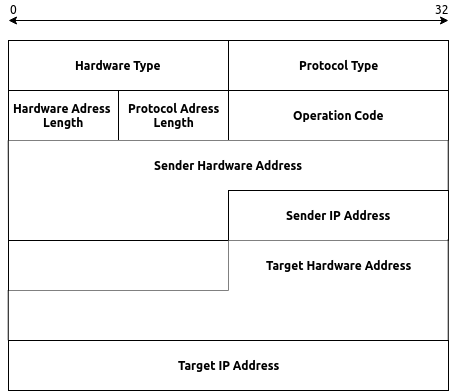
\includegraphics[width=10cm]{arppacket}
  \caption{ARP Paketformat}
  \label{Analyse:ARP Paket}
\end{figure}

\clearpage

Die simple Architektur des \ac{ARP} ermöglicht es, die Kommunikation im Netzwerk zu manipulieren und einen \ac{MitM} Angriff im Netzwerk durchzuführen. Da im Protokoll keine Mechanismen zur Überprüfung der empfangenen Daten wie Checksum o. Ä. vorhanden sind und die Pakete über die Broadcast Adresse im Netzwerk verteilt werden, können die Pakete von jedem Teilnehmer im Netzwerk eingesehen und darauf geantwortet werden. Die Angriffsform des \textit{\ac{ARP} Spoofing} nutzt diese Schwachstelle im Protokoll aus. Der Angreifer versendet gefälschte \ac{ARP} Pakete im Netzwerk. Diese beinhalten die MAC-Adresse der Netzwerkschnittstelle des Angreifers als Zuordnung zu den \ac{IP} Adressen im Netzwerk. Der angegriffene Host sendet die Netzwerkpakete zur im Paket angegebenen \ac{IP} Adresse zukünftig über den Host des Angreifers. Dies lässt den Angreifer die Pakete zwar empfangen, stellt aber die Funktionalität des Netzwerks ein. Um dies zu verhindern, muss der Angreifer die Pakete nun mit Hilfe seiner \ac{ARP} Tabelle zum eigentlichen Empfänger weiterleiten.

Moderne \ac{IDS} können \textit{\ac{ARP} Spoofing} anhand von Mustererkennung identifizieren und Maßnahmen zur Sperre dieser Netzwerkpakete einleiten. Aufgrund der geringen Gültigkeitsdauer des \ac{ARP} Cache ist eine effiziente Erkennung und Vermeidung eines Angriffs in der Praxis nur schwer umzusetzen. Eine weitere Schutzmaßname gegen diese Form des Eingriffs in das Netzwerk kann durch das Arbeiten mit statischen Tabellen erreicht werden. Dies kann jedoch aufgrund des hohen Administrationsaufwands nur in kleinen Netzwerkinfrastrukturen zum Einsatz kommen.

\subsection{\ac{QoS}}
Eine Industrie 4.0 Netzwerkinfrastruktur kann aufgrund der unterschiedlichen Anforderungen an die Systeme auf verschiedenste Weisen ausgeprägt sein. Die Heterogenität der Komponenten im Netzwerk und deren Anforderungen an die Kommunikation auf der vertikalen Ebene der Automatisierungspyramide \autoref{Grundlagen:Automatisierungspyramide} stellen eine Herausforderung für die Sicherheit der Datenübertragung dar und können die Umsetzung eines Netzwerks beeinflussen. Industrie 4.0 Umgebungen können sich über weite Distanzen (\ac{MAN}, \ac{WAN} und \ac{GAN}) erstrecken und sind somit auch von physikalischen Gegebenheiten wie Latenz und Jitter betroffen. Diese Erscheinungen müssen berücksichtigt werden, um eine fehler- und verlustfreie, sichere Kommunikation zu gewährleisten (\cite{torscht2014}).

Für die Beurteilung und Bereitstellung der Dienstgüte in \ac{IP}-Netzen müssen die Übertragungsgüte der Netzzugangsschicht sowie die übertragungstechnischen Parameter der Internetschicht (\ac{IP}-Ebene) betrachtet werden. In IP-Netzen wird der Einfluss auf die \ac{QoS} in den folgenden Parametern beschrieben:

\begin{itemize}
    \item Latenzzeit: Dauer der Paketübertragung
    \item Jitter: Abweichung der Latenzzeit von ihrem Mittelwert
    \item Paketverlustrate: Wahrscheinlichkeit des Verlusts von IP-Paketen während der Übertragung
    \item Durchsatz: gemittelte Datenmenge pro Zeiteinheit
\end{itemize}

All diese Faktoren haben in einem paketorientierten Netzwerk, in welchem die Datenpakete nach dem \textit{Best-Effort-Prinzip} versendet werden, auf die fehlerfreie Kommunikation aufgrund der durch \textit{Ethernet} und \ac{IP} bereitgestellten Fehler- und Flusskontrolle wenig Einfluss. Sie spielen jedoch bei zeitkritischen Anwendungen der Industrie 4.0 eine wichtige Rolle. Auf den niedrigeren Schichten des \ac{TCP}/\ac{IP} Referenzmodells ist es nicht möglich zwischen verschiedenen Datenpaketen der höheren Schichten zu unterscheiden. Um dieses Problem zu lösen werden auf Dienste mit besonderer Güte in \ac{VLAN}s aufgenommen und somit deren Pakete bereits auf der Netzzugangsschicht kenntlich gemacht (\autoref{Analyse:VLAN}), um die Dienstqualität sicherzustellen. Des Weiteren müssen, um \ac{QoS} in einem Netzwerk anzuwenden, diese Mechanismen auf der gesamten Übertragungsstrecke implementiert werden. Der Transport von Daten unterschiedlicher Priorität in Netzwerken wird in \ac{IEEE} 802.1p und \ac{IEEE} 802.1Q\footnote{IEEE Std 802.1Q - IEEE Standard for Local and metropolitan area networks--Bridges and Bridged Networks} beschrieben.

\subsection{IPsec}
Die \ac{IETF} beschreibt im \ac{RFC} 4301\footnote{IETF RFC 4301 - Security Architecture for the Internet Protocol} die Architektur von \ac{IPsec}. \ac{IPsec} ermöglicht es die Schutzziele Vertraulichkeit, Authentizität und Integrität bereits auf der Internetschicht des \ac{TCP}/\ac{IP} Referenzmodells zu umzusetzen. Um alle Schutzziele umzusetzen, wird das Protokoll \ac{IP} um die Bestandteile \ac{AH}, \ac{ESP} und IKE\footnote{IKE - Protokoll zur Verwaltung der Security Association} erweitert.

\ac{IPsec} wurde in der Industrie zur Bereitstellung von dauerhaften Site-to-Site \ac{VPN} Verbindungen genutzt. Aufgrund der immer weiteren Öffnung der Unternehmen und der direkten Kommunikation der Komponenten miteinander finden dauerhafte diese Verbindungsformen in Industrie 4.0 Umgebungen jedoch immer seltener Anwendung. Seit der Verbreitung der Verschlüsselung der Anwendungsdaten über \ac{TLS} werden für die Bereitstellung von getunneltem Netzwerkverkehr aufgrund der besseren Handhabbarkeit und der einfacheren Konfiguration für Administrator und Anwender bevorzugt \ac{SSL}-\ac{VPN} Lösungen verwendet.

Aufgrund der geringen Relevanz der Technik in Industrie 4.0 Netzwerken wird die Kommunikation über das Protokoll \ac{IPsec} im weiteren Verlauf der Thesis nicht weiter untersucht.

\section{Transportschicht}
\label{Analyse:Transportschicht}
Während auf der Netzwerkschicht allein das Protokoll \ac{IP} die Basis für die Vernetzung und Adressierung von Industrie 4.0 Systemen darstellt, wird das Protokoll der Transportschicht durch die Anforderungen an das Netzwerk bestimmt. Der wesentliche Teil der Kommunikation in der Industrie 4.0 erfolgt über ein \ac{IP} Netzwerk, welches zum Datentransport das Protokoll \ac{TCP} für \textit{End2End} (\autoref{Grundlagen:End2End}) Kommunikation nutzt (\cite{sichKom2017}). Wie in \autoref{Grundlagen:Kommunikationsstrukturen} beschrieben, bieten sich in der Praxis bei besonderen Anforderungen wie der Verteilung von Informationen im Netzwerk oder zeitkritischen Automatisierungsanwendungen jedoch auch andere Strukturen für die Kommunikation wie \textit{Publish-Subscribe} (\autoref{Grundlagen:Publish-Subscribe}) in Verbindung mit dem Datagramm \ac{UDP} an. 

Das Protokoll \ac{TCP} sowie das Datagramm \ac{UDP} sind für die Übertragung der Segmente im Netzwerk sowie das Multi-/Demultiplexing verantwortlich. Dabei spielt der Inhalt des zu übertragenden \textit{payload} keine Rolle. Die Analyse der Sicherheit im Netzwerk auf dieser Schicht des \ac{TCP}/\ac{IP} Referenzmodells beschränkt sich ausschließlich auf die Form der Datenübertragung sowie der dafür genutzten Netzlast.

\subsection{\ac{TCP}}
\label{Analyse:TCP}
Das Protokoll \ac{TCP}\footnote{\cite{TCP}} verfolgt das Prinzip eines \textit{guaranteed delivery} und stellt eine zuverlässige Datenübertragung zwischen zwei \textit{Hosts} (\textit{Unicast}) bereit. Hierzu werden verschiedene Mechanismen zur Segmentierung der Daten, dem Verbindungsmanagement sowie der Fehler- und Flusskontrolle bereitgestellt. Diese Mechanismen, welche durch den Aufbau des des \ac{TCP} Headers und die Nutzung von Timeouts und Algorithmen realisiert werden, sind für den Erfolg des Protokolls für zuverlässige, paketorientierte \textit{End2End} Kommunikation verantwortlich.

Ein wichtiger Bestandteil des \ac{TCP} Verbindungsmanagements und der Fehlerkontrolle stellt der 3-Wege-Handshake beim Verbindungsaufbau sowie -abbau dar. Er wird mittels der \textit{Sequence-} und \textit{Acknowledgementnumber} sowie den zugehörigen \textit{Flags} des \ac{TCP} Headers (\ac{SYN}, \ac{SYN-ACK}, \ac{ACK}, \ac{FIN}) realisiert. Während des Verbindungsaufbaus werden die Adresse des Clients sowie der Status der Verbindung im Speicher gehalten. Die folgende Abbildung zeigt schematisch den Ablauf eines \ac{TCP} Verbindungsaufbaus zwischen Client und Server. Der Client sendet zuerst eine Paket mit SYN-Flag zum Server. Dieser bestätigt das eingetroffene Paket des Clients mit dem SYN-ACK Flag, inkrementiert die Sequenznummer x in seinem \textit{acknowledgment number} Segment\footnote{text} und erzeugt eine neue Sequenznummer für das Antwortpaket. Der Verbindungsaufbau wird durch die Bestätigung des SYN-ACK Pakets durch den Client und den Empfang des ACK Pakets vom Server abgeschlossen. Die initiale Sequenznummer x des SYN Pakets sowie die initiale Sequenznummer y des SYN-ACK Pakets können von den Beteiligten frei bestimmt werden. Der 3-Wege-Handshake wird in \autoref{Analyse:TCP Verbindungsaufbau} an einem Verbindungsaufbau von Client zu Server dargestellt.

\begin{figure}[h]
    \centering
    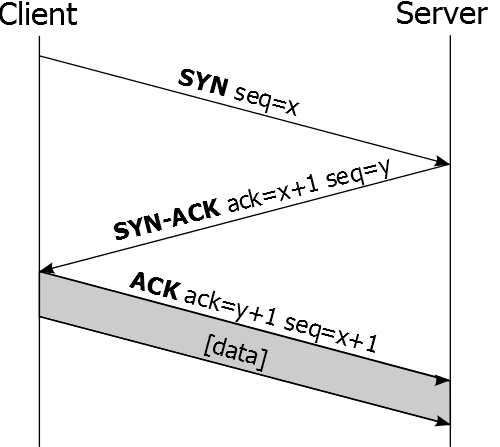
\includegraphics[width=15cm]{tcp-verbindungsaufbau}
    \caption{TCP Verbindungsaufbau}
    \label{Analyse:TCP Verbindungsaufbau}
  \end{figure}
  
\clearpage

\subsubsection{SYN-Flood}
Der Mechanismus des 3-Wege-Handshakes kann durch einen SYN-Flood Angriff ausgenutzt werden und somit die Netz- und Systemlast manipuliert werden. Der SYN-Flood stellt eine Form des \ac{DoS} bzw. \ac{DDoS} Angriffs dar. Dabei werden zu einem gezielten \ac{TCP} Dienst große Menge an Paketen mit gesetztem SYN \textit{Flag} gesendet, um einen Verbindungsaufbau zum Server vorzutäuschen. Nach Erhalt des Pakets sendet der Server dem Client ein SYN-ACK Paket um den Verbindungsaufbau zu initiieren und wartet auf Bestätigung. Diese Bestätigung wird vom Angreifer unterschlagen. Somit bleiben auf dem angegriffenen System Ressourcen dieser halb offenen Verbindung bis zum erreichen eines Timouts belegt. Ein verteilter Angriff auf ein System kann dessen Ressourcen schnell komplett beanspruchen und somit zur Ablehnung jeglicher weiterer Verbindungen führen.

Die Kritikalität dieses Angriffs liegt in der Unausgewogenheit der benötigten Ressourcen zwischen Angreifer und Opfer. Es benötigt nur wenig Rechenaufwand und Bandbreite um ein 20 Byte großen \ac{TCP}-SYN Header mit entsprechender \textit{payload} zu erzeugen und zu versenden, jedoch viele Ressourcen um sich durch eine Echtzeitanalyse der Pakete durch eine Firewall oder SYN-Cookies vor diesen Angriffen zu schützen. Diese werden aufgrund ihrer Ressourcenbelastung aus wirtschaftlichen Gründen meist nur minimal oder gar nicht umgesetzt.

Der Mechanismus der SYN-Cookies wird auf dem Server implementiert. Hierbei werden die Informationen Zeitstempel, \ac{IP} Adresse und Port von Client und Server in die initiale Sequenznummer des vom Server gesendeten SYN-ACK Pakets kodiert. Diese müssten normalerweise in einer Tabelle im Speicher gehalten werden. Ein überlaufen der Tabelle ist somit unmöglich, da sie nicht vorhanden ist. Jedoch benötigt jede Kodierung und Dekodierung Systemressourcen. Ein ausreichend großer Angriff auf das System kann somit trotzdem die gesamten Systemressourcen beanspruchen und das Ziel eines \ac{DDoS} Angriffs, der Negierung eines Dienstes, erfüllen.

Dedizierte Firewalls können mit Hilfe von \ac{IDS} die Pakete beim Eintreffen im Netzwerk analysieren, Angriffe erkennen und Verbindungen dieser Quelladressen blockieren.

\subsubsection{Sockstress}
Eine weitere Angriffsform, welche den 3-Wege-Handshake des \ac{TCP} Protokolls als Mis-Use-Case nutzt, wurde im Jahr 2008 von den Sicherheitsforschern Jack C. Louis und Robert E. Lee von Outpost24\footnote{http://www.outpost24.com} entdeckt und mit dem Namen \textit{sockstress} bezeichnet. Der Angriff stellt eine einfache Form eines \ac{DoS} Angriffs dar. Das Ziel dieses Angriffs ist, ähnlich wie beim SYN-Flood, eine Negierung eines Dienstes oder des gesamten Systems mit Hilfe asymmetrischer Ressourcenauslastung bei Angreifer und Opfer zu erzielen.

Im Gegensatz zum SYN-Flood stellt \textit{sockstress} eine vollständige Verbindung zum Server über den 3-Wege-Handshake her. In der einfachsten Form des Angriffs wird das \textit{Receive Window} Flag des \ac{TCP} Headers im ersten \ac{TCP} Segment, welches vom Client zum Server nach dem Verbindungsaufbau übertragen wird, auf 0 gesetzt. Dies bedeutet, dass der Client dem Server mitteilt, dass er im Moment keine weiteren Daten empfangen kann. Der Server wird, durch den abgeschlossen Verbindungsaufbau, gezwungen die Verbindung im Speicher zu halten und den Client periodisch zu prüfen, ob dieser Daten empfangen kann. Dies belegt Systemressourcen und kann genutzt werden, um einen Dienst oder ein System zum Ablehnen aller Verbindungen oder zum Absturz zu bewegen. Der Ablauf des Angriffs wird in \autoref{Analyse:Sockstress-Sequenzdiagramm} in Anlehnung an ein \ac{UML}-Sequenzdiagramm schematisch dargestellt. Die Nutzung von SYN-Cookies hat bietet keinen Schutz gegen diese Form des Angriffs, da die Verbindung vom Client zum Server vollständig aufgebaut wird. Industrieanlagen müssen mit Hilfe externer \ac{DDoS} Serviceanbieter wie Akamai\footnote{Link - https://www.akamai.com} oder Cloudflare\footnote{Link - https://www.cloudflare.com}, Firewalls und \ac{IDS} Systeme oder spezieller Appliances, welche den Netzwerkverkehr Netzwerk-, Transport- und Anwendungsschicht überwachen, geschützt werden.

\begin{figure}[h]
  \centering
  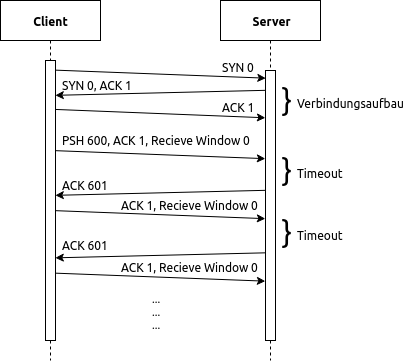
\includegraphics[width=15cm]{sockstress}
  \caption{Sockstress Sequenzdiagramm}
  \label{Analyse:Sockstress-Sequenzdiagramm}
\end{figure}

\clearpage

\subsection{\ac{UDP}}
Das von der \ac{IETF} im \ac{RFC} 768\footnote{Link - https://tools.ietf.org/html/rfc768} definierte Datagramm \ac{UDP} ist ein verbindungsloses\footnote{verbindungslos - TODO}, nicht-zuverlässiges\footnote{nicht zuverlässig - TODO} Übertragungsprotokoll. Der \ac{UDP} Header ist im Gegensatz zum \ac{TCP} Header (20 Bytes) nur 8 Byte lang und bietet somit einen sehr geringen \textit{Overhead}\footnote{Overhead - TODO} beim Versenden von \ac{IP} Paketen. \ac{UDP} wurde als Alternative zu \ac{TCP} entwickelt, um die Kommunikation mit niedrigeren Latenzen für Dienste wie \ac{SNMP} oder \ac{DNS}oder \ac{VoIP} zu ermöglichen (\cite{UDP2003}). Es wird auf den für die Latenz kritischen 3-Wege-Handshake verzichtet und das \textit{Fire-and-Forget}\footnote{Fire-and-Forget - TODO} Prinzip angewandt, wobei keine Verbindung zwischen zwei Kommunikationspartnern hergestellt wird, sondern die Pakete ohne Flusskontrolle von Sender zu Empfänger gesendet werden.

\ac{UDP} findet in vielen Industrienetzen Einsatz als Transportprotokoll. Es bietet sich, vor allem durch seine Simplizität und den geringen Overhead im Netzwerk für die Informationsverteilung mit niedrigen Latenzzeiten an. Durch die Broad- und Multicast Funktionalitäten des \ac{UDP} ist es möglich über das in \autoref{Grundlagen:Publish-Subscribe} beschriebene \textit{Publish Subscribe} Muster zu kommunizieren und somit die Netzlast bei einer großen Anzahl von Empfängern gering zu halten.

\ac{UDP} führt keine Validierung der Absenderadresse im Paketheader durch (\cite{UDP2003}). Dies ermöglicht die Anwendung von \ac{IP} Spoofing. \ac{IP} Spoofing kann genutzt werden, um \ac{DoS} bzw. \ac{DDoS} Angriffe auf ein System durchzuführen. Eine Untersuchung des Netzwerkdienstes \ac{DNS}, welcher auf der Nutzung des Transportprotokolls \ac{UDP} basiert, wird in \autoref{Analyse:DNS} beschrieben und durchgeführt.

\section{Anwendungsschicht}
\label{Analyse:Anwendungsschicht}
Die Netzwerkkommunikation der Anwendungsschicht in Industrie 4.0 Umgebungen basiert auf dem \ac{IP} der Internetschicht. Um die Integration und Verwaltung der Netzwerkteilnehmer zu erleichtern, werden \ac{IP} basierende Dienste wie \ac{DNS} für die Namensauflösung sowie \ac{DHCP} für die Adressvergabe und das Routing genutzt. Die Anwendungsschicht des \ac{TCP}/\ac{IP} Referenzmodells wird durch eine Vielzahl von Protokollen beschrieben. Bestehende Lösungen des \ac{IoT} nutzen Protokolle wie \ac{HTTP}, \ac{XMPP} oder \ac{SMTP} zur Kommunikation über das Netzwerk. In der \ac{M2M} Kommunikation des \ac{IIoT} haben sich die Protokolle und Standards \ac{OPC UA}, \ac{DDS}, \ac{MQTT} und \ac{CoAP} für unterschiedliche Anforderungen an die Netze und deren Teilnehmer hervorgetan. 

\subsection{\ac{DNS}}
\label{Analyse:DNS}
\ac{DNS} wird von der \ac{IETF} in den \ac{RFC} 1034\footnote{Domain Names – Concepts and Facilities}, 1035\footnote{Domain Names – Implementation and Specification}, 2181\footnote{Clarifications to the DNS Specification} und 2782\footnote{A DNS RR for specifying the location of services (DNS SRV)} beschrieben und verwaltet. Es stellt einen hierarchischen Verzeichnisdienst für \ac{IP}-Netze zur Verfügung. 

Eine der Hauptaufgaben des \ac{DNS} ist der \textit{forward lookup}. Hierbei werden Domain- bzw. Hostnamen in \ac{IP}-Adressen übersetzt. Das Zusammenspiel eines hierarchischen Verzeichnisdienstes und der Namensauflösung bietet Angriffsfläche zum Eingriff auf die Kommunikation im Netzwerk. Im folgenden werden bekannte Angriffsformen auf den \ac{DNS} Dienst und deren Auswirkungen auf das Netzwerk beschrieben.

\subsubsection{\ac{DNS} Spoofing}
Die Angriffsmethode des \ac{DNS} Spoofing verfolgt, ähnlich wie \textit{Cache Poisoning}\footnote{TODO - Cache Poisoning}, das Ziel gefälschte \ac{RR} in den \ac{DNS} Cache des Opfers einzuschleusen. Während das \textit{Cache Poisoning} aus einer Softwareschwachstelle hervorging, bei der zusätzliche, gefälschte \ac{DNS} Einträge zu korrekten \ac{DNS} Antworten hinzugefügt wurden und somit der Cache eines Nameservers kompromittiert wurde, befindet sich der Angriffsvektor beim \ac{DNS} Spoofing in der Fälschung von \ac{DNS} Antworten. Die Header der Netzwerkpakete werden mit Hilfe von \textit{IP Spoofing}\footnote{TODO - IP Spoofing bezeichnet das Versenden von IP Paketen mit gefälschter Absender IP} so manipuliert, dass sie vorgeblich vom \textit{authorativen} Nameserver stammen. 

Um \ac{DNS} Spoofing erfolgreich durchzuführen muss die gefälschte \ac{DNS} Response des Angreifers vor der Antwort des zuständigen Nameservers beim angegriffenen \ac{DNS} Resolver eintreffen. Sobald der physikalische Zugang zum Netzwerk gewährleistet ist, können die Latenzzeiten der gefälschten Pakete im Netzwerk sehr gering gehalten werden. Ist dies nicht möglich, kann mit Hilfe eines \ac{DoS} bzw. \ac{DDoS} Angriffs auf den zuständigen Nameserver, dessen Antwortzeit beeinflusst werden. Des weiteren muss die ID im \ac{DNS} Header mit der des Request übereinstimmen. Dies wird in \autoref{Analyse:DNS Request Response} dargestellt und kann mit Hilfe des Netzwerkanalysetools Wireshark\footnote{TODO Link zu Wireshark} in einer beliebigen Netzwerkumgebung mit zuständigem \ac{DNS} Server nachgewiesen werden. Auf der linken Seite ist ein DNS Request eines Hosts im Netzwerk und dessen \ac{DNS} Header mit ID zu erkennen. Auf der rechten Seite ist die Antwort des im Netzwerk vorhandenen \ac{DNS} Nameservers zu sehen. Request und Response müssen die gleiche ID besitzen, um als gültig betrachtet zu werden.

\begin{figure}[h]
    \centering
    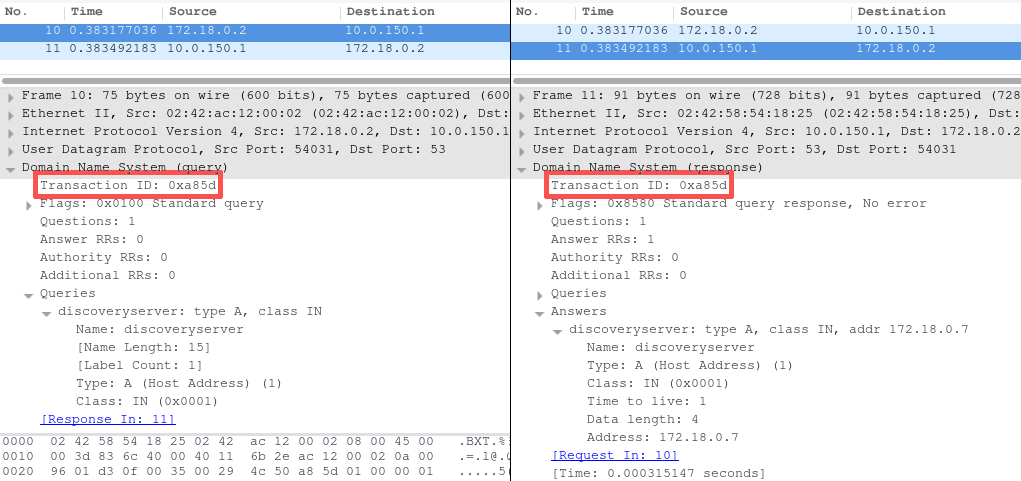
\includegraphics[width=15cm]{dns-response-request}
    \caption{Wireshark - ID im DNS Header}
    \label{Analyse:DNS Request Response}
  \end{figure}
  
\clearpage

\subsubsection{\ac{DNS} Amplification}
\label{Analyse:DNS Amplification}
Eine Form eines \ac{DDoS} Angriffs (\autoref{Analyse:DoS/DDos}) ist über \ac{DNS} möglich und wird \ac{DNS} Amplification genannt. Bei der \ac{DNS} Amplification werden \ac{DNS} Anfragen an offene Nameserver gesendet und mit Hilfe von \ac{IP} Spoofing als Quell-\ac{IP} die Adresse des Angreifers genutzt. Somit treffen die \ac{DNS} Antworten beim anzugreifenden System ein und belasten dieses durch erhöhten Rechenaufwand sowie dessen Netzwerk durch Traffic. Ein weiterer Seiteneffekt dieses Angriffs ist eine hohe Last der Nameserver, welches durch das rekursive Verhalten der \ac{DNS} Namensauflösung hervorgerufen wird. \ac{DNS} Amplification beschreibt eine Form des \ac{DRDoS}.

Mit der Erweiterung des \ac{DNS} in der \ac{IETF} \ac{RFC} 2617\footnote{Link - https://www.ietf.org/rfc/rfc2671.txt} wurde es notwendig, die Größe der \ac{DNS} Antworten von 512 Byte auf einen dynamischen Puffer bis über 4000 Bytes zu erhöhen, um zusätzliche Informationen und Flags wie \autoref{Analyse:DNSSEC} über das \ac{DNS} übertragen zu können. Dies wird sich vom Angreifer zunutze gemacht, da an den Nameserver Requests mit einer Paketgröße von 60 Bytes gesendet werden können, welche eine Antwort mit 4000 Bytes und mehr provozieren und somit einen \ac{BAF}\footnote{BAF - Verhältnis von Eingangs- zum Ausgangssignal} von ca. 66 im Netz haben (\cite{Ledermueller2009}). Dieser wird bei \ac{DNS} Amplification durch die Paketgröße der Anfrage sowie der Antwort dargestellt.

\autoref{Analyse:DNS Amplification Beispiel} stellt die Funktionsweise eines mit Hilfe von \ac{DNS} Amplification durchgeführten \ac{DDoS} Angriffs dar. Der Angreifer (links) sendet zum offenen Nameservern gefälschte \ac{DNS} Anfragen mit Quelladresse des Opfers (rechts). Der Nameserver erfragen beim \textit{authorativen} Nameserver die Zone, dieser stellt die erfragten \ac{RR} bereit, anschließend sendet der Nameserver dem Opfer die Antworten zu.

\begin{figure}[h]
    \centering
    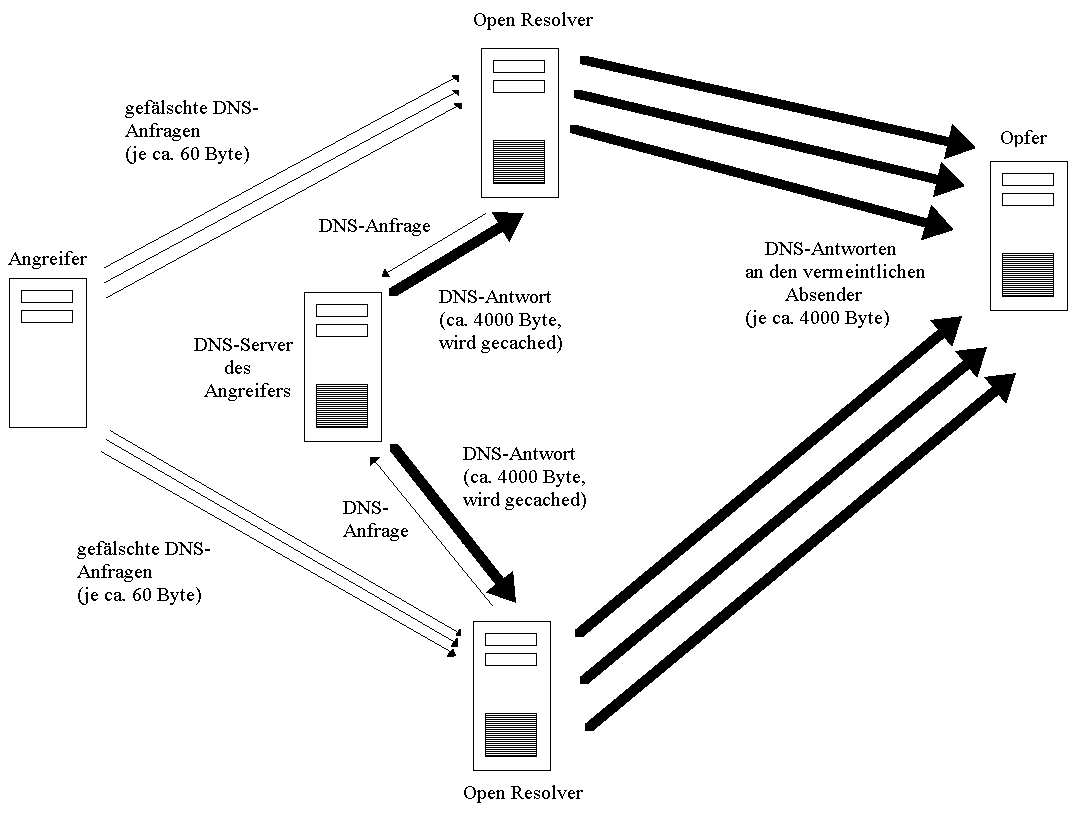
\includegraphics[width=15cm]{dns-amplification}
    \caption{Schematisches Beispiel: DNS Amplification}
    \label{Analyse:DNS Amplification Beispiel}
  \end{figure}
  
\clearpage

Diese Form des Angriffs kann aus dem internen Netz sowie von extern auf öffentlich zugängliche Systeme durchgeführt werden. \ac{DoS} Attacken stellen besonders für Industrie 4.0 Netzwerke, deren komplexe Kommunikation und Anforderungen eine hohe Bedrohung dar. Durch den erheblichen \ac{BAF} können diese Angriffe mit wenig Bandbreite beim Angreifer durchgeführt werden und gleichzeitig das Netzwerk des Opfers voll auslasten. Wie in \autoref{Analyse:DNS Amplification am Beispiel von isc.org} dargestellt, kann durch die Abfrage der Zone \textit{isc.org} eine 3385 Byte große Antwort vom Nameserver provoziert werden. Dies führt zu einem \ac{BAF} von ca. 56. \autoref{Analyse:Netzlast bei DNS Amplification} beschreibt die Netzlast während eines \ac{DNS} Amplification Angriffs im Quell- und Zielnetz. Auf der X-Achse wird die Anzahl der gesendeten Pakete pro Sekunde dargestellt, die Y-Achse zeigt die Netzlast in Gigabit pro Sekunde. Es ist eine lineare Steigerung der Netzlast in beiden Netzen zu erkennen, entscheidend ist jedoch der \ac{BAF}. Beim Versandt von 10000 Paketen pro Sekunde müssen im Quellnetz nur ca. 4,8 Megabit/s an Daten transferiert werden, im Zielnetzwerk wird mit 287 Megabit/s eine wesentlich höhere Last erzeugt. Es ist möglich, mit einer vergleichsweise geringen Bandbreite im Quellnetz ein Netzwerk mit hoher Bandbreite im Zielnetz auszulasten.

\begin{figure}[h]
    \centering
    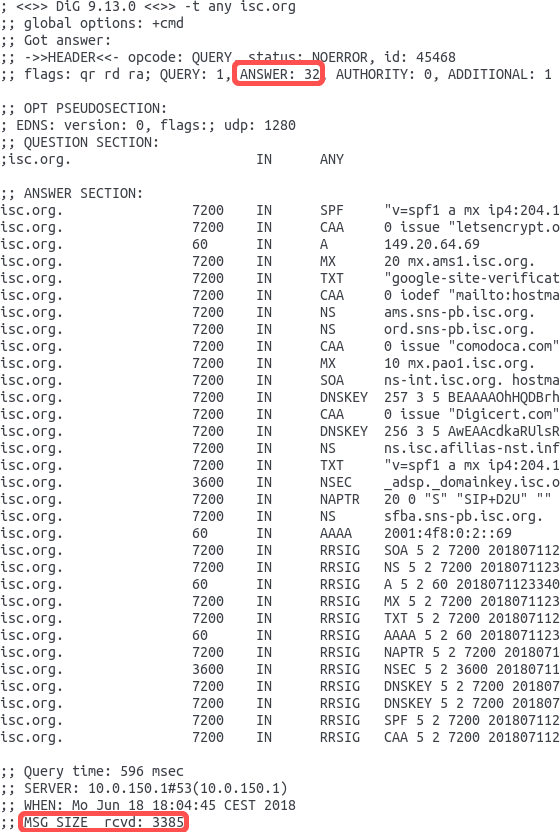
\includegraphics[width=10cm]{dig-dnsamplification}
    \caption{DNS Amplification am Beispiel von isc.org}
    \label{Analyse:DNS Amplification am Beispiel von isc.org}
\end{figure}

\begin{figure}[h]
    \centering
    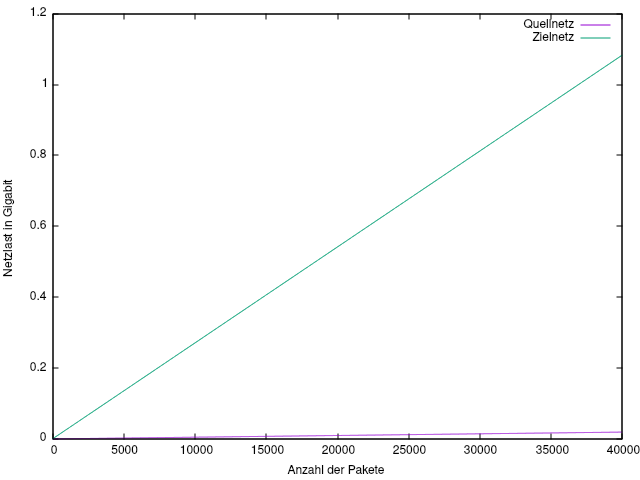
\includegraphics[width=15cm]{gnuplot-dnsamplification}
    \caption{Netzlast bei DNS Amplification}
    \label{Analyse:Netzlast bei DNS Amplification}
\end{figure}
  
\clearpage

Der \ac{DNS} bietet weitere Angriffsmöglichkeiten wie \ac{DNS} Fast Fluxing oder \ac{DNS} Information Leakage. Diese Angriffe dienen zum \textit{Phishing} von Daten oder der Spionage der Netzwerkstruktur. Sie nehmen initial keinen Einfluss auf den Netzwerkverkehr und dienen der Vorbereitung von Folgeangriffen und dem Sammeln von Informationen. Die Analyse der Sicherheit der Netzwerkkommunikation beschränkt sich auf Angriffe, welche direkten Einfluss in die Kommunikation im Netzwerk haben.

Das \ac{DNS} kann um zusätzliche Sicherheitsmechanismen wie \ac{TSIG} und \ac{DNSSEC} erweitert werden, um einen Schutz vor Eingriffen in die Namenauflösung zu gewährleisten. Diese bieten die Möglichkeit die Kommunikation zwischen Nameservern und Resolvern zu sichern, die Authentizität sowie die Validität der Zonen sicherzustellen. Bei \ac{TSIG} werden symmetrische Schlüssel während der Übertragung der Domainzonen genutzt, \ac{DNSSEC} benötigt die Verwendung von Extended \ac{DNS}\footnote{TODO - Extended DNS} und erweitert die Zonen der Domains um zusätzliche \ac{RR}. Diese beinhalten den öffentlichen Schlüssel eines asymmetrischen Schlüsselpaars. Der private Schlüssel liegt beim \textit{authorativen} Nameserver der Zone. Durch die Signierung der Zonen ist deren Authentizität geschützt. Alle im Internet vorhandenen Root-Nameserver\footnote{TODO - Root-Nameserver} nutzen die \ac{DNS} Erweiterung \ac{DNSSEC}. In internen Netzen werden diese Sicherheitsmaßnahmen aufgrund von zusätzlichem Aufwand meist nicht umgesetzt (\cite{Ledermueller2009}).

\subsection{\ac{DHCP}}
\label{Analyse:DHCP}
\ac{DHCP} ist von der \ac{IETF} im \ac{RFC} 2131\footnote{Link - https://www.ietf.org/rfc/rfc2131.txt} definiert. Es stellt ein Framework zur Bereitstellung von Host-Konfigurationsparamertern in einem \ac{TCP}/\ac{IP} Netzwerk dar. Dazu gehören die \ac{IP} Adresse, Netzmaske, Gateway sowie zuständiger \ac{DNS} des Clients. Da ein neuer Client im Netzwerk keine Informationen über die vorhandenen Clients und dessen Topologie besitzt, muss er, um die Konfigurationsparameter für das Netzwerk zu erhalten (\ac{DHCP} Discover), über einen Broadcast im Netzwerk nach Adressangeboten fragen. Der \ac{DHCP} Discover findet über das Transportprotokoll \ac{UDP} statt.

Der Mangel an Informationen bei der initialen Verbindung eines Clients im Netzwerk, kann von einem Angreifer genutzt werden, um die Netzwerkkonfiguration zu manipulieren. Da der Broadcast des Clients an das gesamte Netzwerk versandt wird, ist es dem Angreifer möglich selbst auf diese Anfrage zu antworten. Hierzu wird die Technik des Spoofing in Verbindung mit \ac{ARP} Poisoning oder einem zusätzlichen \ac{DHCP} Server (Rogue \ac{DHCP}), welcher vom Angreifer kontrolliert wird, im Netzwerk genutzt. In diesem Fall muss es dem Angreifer nur gelingen schneller auf den \ac{DHCP} Discover bzw. \ac{DHCP} Request des Clients zu antworten als der zuständige \ac{DHCP} Server. Somit kann die Netzwerkkonfiguration des Clients manipuliert werden.

Ein Angriff auf das \ac{DHCP} in Netzwerken kann weitreichende folgen für die Netzwerksicherheit mit sich bringen. Durch die Änderung der Client-Adressen und Subnetze kann es zu \ac{IP} Adresskonflikten im Netzwerk kommen und die Kommunikation beschränkt bzw. stillgelegt werden. Größere Auswirkungen auf die Netzwerksicherheit stellt das Umlenken des Datenverkehrs durch Manipulation der \ac{DNS}- bzw. Gateway-Parameter dar. Hierbei kann der gesamte Netzwerkverkehr eines Clients umgelenkt werden, um einen \ac{MitM} Angriff durchzuführen und den Netzwerkverkehr auszulesen.

Da das \ac{IP} Hilfsprotokoll \ac{DHCP} keine Sicherheitsmaßnahmen zur Verhinderung dieser Angriffe mit sich bringt, ist es notwendig sich vor diesen Bedrohungen schon auf den unteren Schichten des \ac{TCP}/\ac{IP} Referenzmodells zu schützen. Eine in der Industrie weit verbreitete Technik zum verhindern von Angriffen auf das \ac{DHCP} wird bereits in der Netzzugangsschicht umgesetzt. Netzwerkkomponenten wie Router und Swichtes werden mit Hilfe von \ac{DHCP} Snooping konfiguriert, welches es ermöglicht \ac{DHCP} Nachrichten zu überwachen und diese nur von vertrauenswürdigen Ports in das Netzwerk weiterzuleiten. Somit werden \ac{DHCP} Pakete, welche von einem im Netzwerk eingeschleusten Rogue \ac{DHCP} Server verteilt werden direkt verworfen und nehmen keinen Einfluss auf das bestehende Netzwerk.

\subsection{\ac{OPC UA}}
\label{Analyse:OPC UA}
Die \ac{OPC UA} beschreibt ein mehrschichtiges, generisches Sicherheitskonzept, welches \textit{Transport Layer}, \textit{Communication Layer} und \textit{Application Layer} umfasst. Die Kommunikation des Protokolls \ac{OPC UA} wird während des Nachrichtenaustauschs über eine \ac{UA} \textit{Secure Conversation} durchgeführt. Diese wird vom Netzwerkstack, dem in der Transportschicht genuntzten Protokoll, dem \textit{Secure Channel} sowie der \textit{Session} der Anwendungsschicht (\autoref{Analyse:OPC UA Security Architecture}) bestimmt. (\cite{opcpt2})

In der \textit{Session} werden die Sicherheitsbestandteile Benutzerauthentifizierung und Benutzerauthorisierung umgesetzt sowie die Nutzdaten übertragen (\cite{opcpt2}). Die auftretenden Daten werden zur Übertragung an den \textit{Communication Layer} übergeben. Die Sicherheit der \textit{Session} basiert somit auf den Gegebenheiten des \textit{Secure Channel} im \textit{Communication Layer}. Die Form der Nachrichten im \textit{Secure Channel} wird durch die \textit{Security Policy} im gewählten \textit{Message Security Mode} bestimmt. 

\begin{figure}[h]
  \centering
  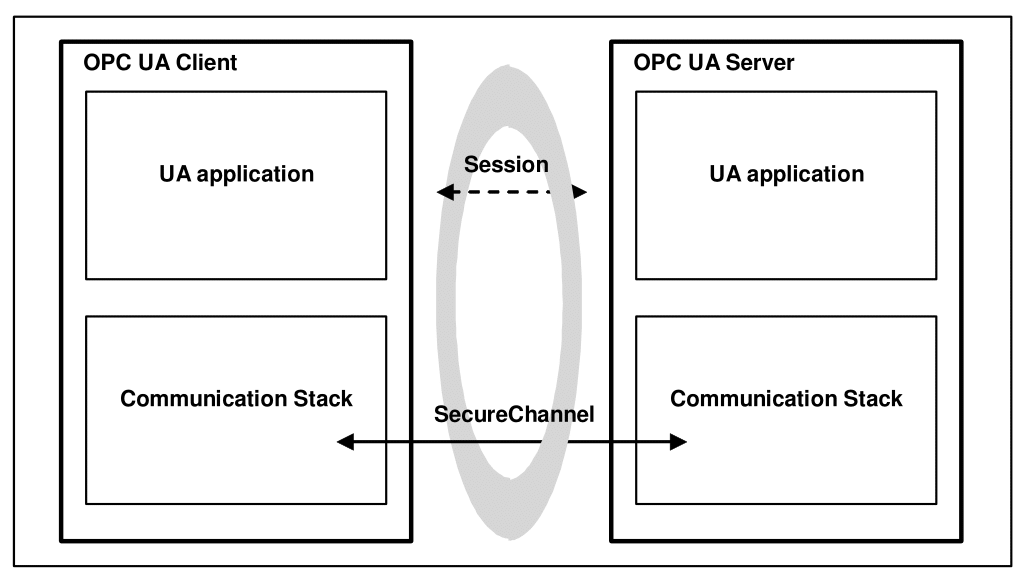
\includegraphics[width=10cm]{opcua-securechannel}
  \caption{OPC UA Security Architecture} 
  \label{Analyse:OPC UA Security Architecture}
\end{figure}

\clearpage

Aufgrund der verschiedenen Anforderungen der Industrie an ihre Systeme werden von \ac{OPC UA} mehrere \textit{Security Policies} im \textit{Secure Channel} zur Informationsübertragung zur Verfügung gestellt. Dies ist notwendig, da die Verwendung von Verschlüsselungsalgorithmen und Kodierungsverfahren Ressourcen benötigt und Latenzen verursacht, welche unter Umständen nicht vorhanden sind oder nicht geleistet werden können. Eine Fehlkonfiguration des Protokolls kann jedoch Auswirkungen auf den Betrieb des Netzwerks und der Komponenten haben sowie die Integrität der Daten gefährden. Die Bezeichnungen der geöffneten Verbindungen können irreführend sein, da bei der Verwendung der \textit{Security Policy} "`none"' zwar ein \textit{Secure Channel} hergestellt wird, welcher jedoch keine Sicherheitsprofile bereitstellt und somit die unverschlüsselte Kommunikation der Komponenten zulässt (\cite{opcpt7}).

Auf der Transportschicht beschreibt die Spezifikation von \ac{OPC UA} mit dem \ac{UACP} ein abstraktes Protokoll zur Herstellung einer Vollduplexverbindung in einer Client-Server Architektur. Implementierungen dieses Protokolls können über jede Middleware, welche den Austausch von Nachrichten im Vollduplexverfahren über \ac{TCP}/\ac{IP} und \textit{Websockets} unterstützt, durchgeführt werden. Somit ist das von \ac{OPC UA} spezifizierte Protokoll für die Zukunft flexibel. Die Spezifikation des abstrakten Protokolls \ac{UACP} wird im 5. Teil der \ac{OPC UA} Spezifikation\footnote{OPC Unified Architecture Specification Part 6: Mappings} (\cite{opcpt5}) beschrieben und beinhaltet die Form der Nachricht, den Verbindungsaufbau, die Kommunikation und die Fehlerbehandlung.

Die \textit{Transport Layer Security} stellt die Sicherheit auf Nachritenebene her und erfüllt die Schutzziele Authentifizierung, Integrität und Vertraulichkeit. Um dies zu ermöglichen, werden verschiedene Transport- sowie Anwendungsprotokolle im Verbund genutzt. Die Sicherheitsmechanismen der Anwendungsschicht dienen der Bereitstellung der Authorisierung und Authentifizierung der Benutzer.

In \autoref{Analyse:OPC UA Kommunikationswege} werden die von \ac{OPC UA} bereitgestellten Protokollstacks beschrieben. Diese bestehen aus einer Verbindung von \ac{TCP} auf Transportebene und dem \ac{UA} Binary Protokoll zur Kodierung der Nachrichten, einem Webservice über \ac{HTTP} bzw. \ac{HTTPS} und \ac{SOAP} mit \ac{XML} Encoding oder einer hybriden Form aus beiden. Alle Kommunikationsformen beinhalten mit \ac{UA} Secure Conversation, \ac{TLS} und \ac{WS} Sercure Conversation ein Sicherheitsmodell auf Transport- oder Nachrichtebene. Die Nutzung von Webtechnologien sowie eines binären Protokolls ermöglicht eine hohe Kompatibilität und flexible Anwendungsmöglichkeiten des Protokolls in Umgebungen mit unterschiedlichen Anforderungen.

\begin{figure}[h]
  \centering
  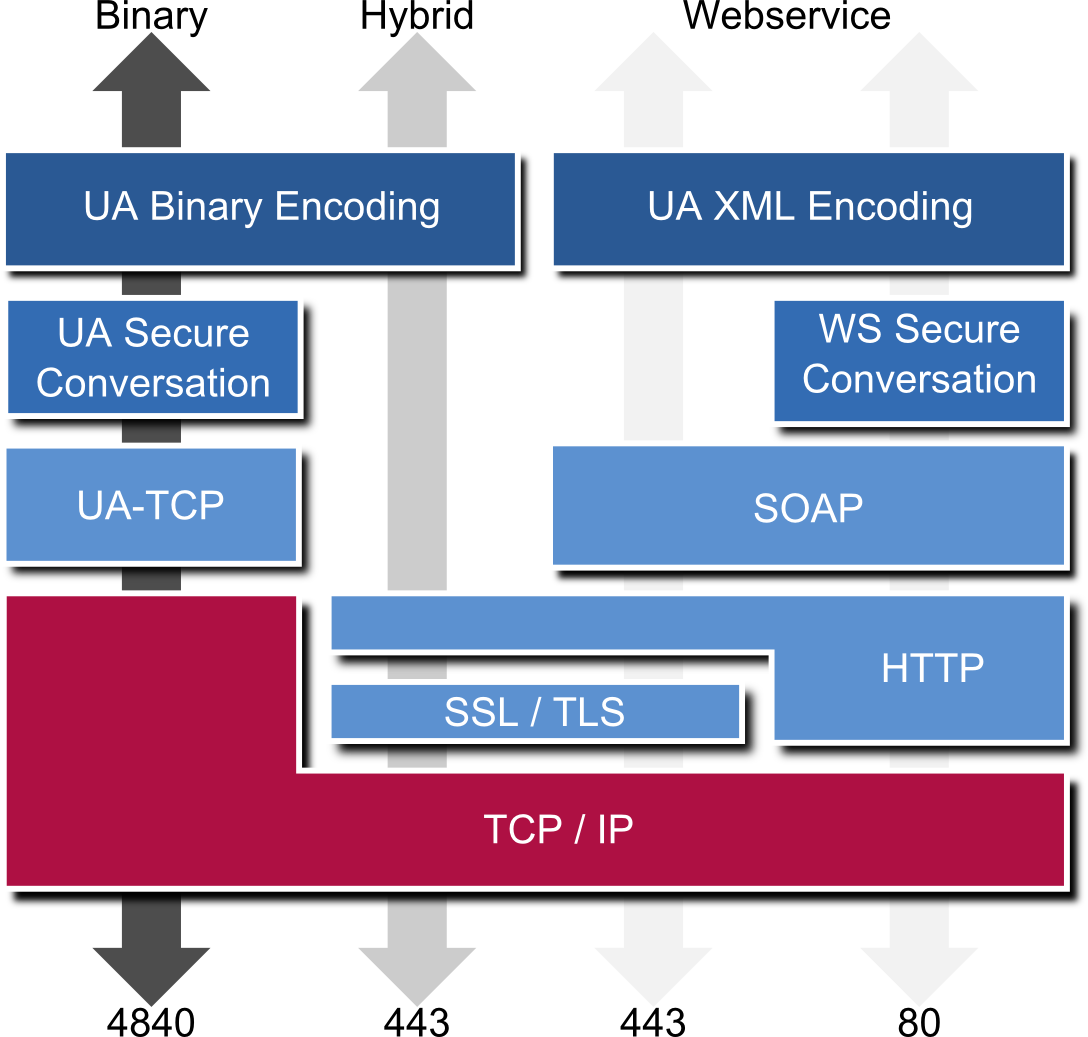
\includegraphics[width=10cm]{opcuaprotocol}
  \caption{OPC UA Kommunikationswege} 
  \label{Analyse:OPC UA Kommunikationswege}
\end{figure}

\clearpage

Die beschriebenen Protokollstacks (\autoref{Analyse:OPC UA Kommunikationswege}) bilden mit ihren Sicherheitsmechanismen die Grundlage für eine sichere Datenübertragung. Die Form der Datenübertragung über \ac{SOAP}/\ac{HTTP} wurde ab Version 1.03 der Spezifikation als veraltet angesehen, da es in der Industrie nicht umgesetzt wurde (\cite{opcpt5}) und wird im weiteren Verlauf der Thesis nicht beschrieben. Die Protokolle \ac{UA} Binary über \ac{TCP} und die Hybridform aus den Protokollen \ac{UA} Binary und \ac{HTTPS} Webservice werden produktiv genutzt und im folgenden näher erläutert.

\subsubsection{\ac{UA} Binary über \ac{TCP}}
Das \ac{UA} Binary Protokoll über \ac{TCP} wird für Kommunikation mit optimierter Geschwindigkeit und Durchsatz genutzt. Es besitzt den geringsten Overhead sowie Ressourcenverbrauch, da kein zusätzlicher Parser für \ac{HTTP} oder \ac{XML} genutzt werden muss und somit die Systemlast gering gehalten werden kann. Die sichere Kommunikation wird erst auf Nachrichtenebene durch die \ac{UA} Secure Conversation hergestellt. Für die Transportebene gelten durch das genutzte Protkoll \ac{TCP} weiterhin die Bedrohungen von \autoref{Analyse:TCP}.

\subsubsection{\ac{UA} Binary über \ac{HTTPS}}
Die Hybridform der Kommunikation über einen \ac{HTTPS} Webservice mit Hilfe der \ac{UA} Binary Protokolls vereint die Vorteile des Ressourcenschonenden \ac{UA} Binary Protokolls über \ac{TCP} und die weitreichende Kompatibilität eines Webservice. Die Sicherheit der Netzwerkkommunikation wird auf der Transportebene mit Hilfe von \ac{TLS} hergestellt.

In der aktuellen Version des \ac{OPC UA} Protokolls wird die Transportsicherheit mit \ac{TLS} 1.2 und der Cipher Suite \textit{TLS RSA WITH AES 256 CBC SHA256} bereitgestellt (\cite{opcpt7}). Hierbei ist zu beachten, dass die Rechenleistung der Systeme wächst und somit Verschlüsselungsalgorithmen mit der Zeit unsicher werden. Eine \ac{TLS} Verbindung mit schwacher Cipher Suite stellt keine sichere Verbindung bereit. Des Weiteren wurden in den Implementierungen von \ac{TLS} bereits schwerwiegende Fehler verursacht, welche die Transportsicherheit wie z. B. im Falle von \textit{Heartbleed}\footnote{TODO - Link zu Heartbleed} einschränken können.

Eine weitere Bedrohung stellt das genrelle Verfahren der Ausstellung von Zertifikaten bereit. Diese Zertifikate werden von Dienstleistern ausgestellt, welche als vertrauenswürdig eingestuft und als Root-\ac{CA} bezeichnet werden. Die Herstellung der Vertrauenswürdigkeit eines Ausstellers liegt im Ermessen des Softwareherstellers und dessen Aufnahme in die Liste vertrauenswürdiger \ac{CA}. 

Die Verwaltung der Zertifikate im Netzwerk kann, um ein erhöhtes Maß an Sicherheit zu gewährleisten, durch Bereitstellung einer \ac{CA}, \ac{RA} und \ac{VA} im Netzwerk selbst Umgesetzt werden. Diese Bestandteile beschreiben eine \ac{PKI}. Sie dient der Erzeugung, Verteilung, Überprüfung, Verwaltung und Speicherung der öffentlichen sowie privaten, asymmetrischen Schlüssel und Zertifikate. Die intern erstellten und genutzten Zertifikate können erst für die Kommunikation mit externen Partnern genutzt werden, wenn dieser die \ac{CA} des Unternehmens als vertrauenswürdig einstuft. Geschieht dies nicht, ist die Herstellung einer vertrauenswürdigen Verbindung nur über ein Zertifikat eines akkreditierten Zertifizierungsdienstanbieters möglich.

\subsection{\ac{CoAP}}
Um den in \autoref{Grundlagen:IoT/IIoT} beschriebenen Einsatzmöglichkeiten in ressourcenbeschränkten Umgebungen sowie der \ac{M2M} Kommunikation gerecht zu werden, stellt das Protokoll mehrere Mechanismen zur Verfügung.

Der Header des Protokolls \ac{CoAP} besteht aus 32 Bit. Dieser wird von einem \textit{Token}, weiteren \textit{Options} Parametern sowie dem \textit{Payload} gefolgt. \ac{CoAP} basiert auf dem Transportprotokoll \ac{UDP}. Der minimale Header sowie die Nutzung von \ac{UDP} ermöglicht die Übertragung der Nutzdaten im Netzwerk mit geringem Overhead und halten die Last bei häufiger Kommunikation der Komponenten gering. Das Nachrichtenformat des \ac{CoAP} Protokolls wird in \autoref{Analyse:CoAP Message Format} dargestellt.

\begin{figure}[h]
  \centering
  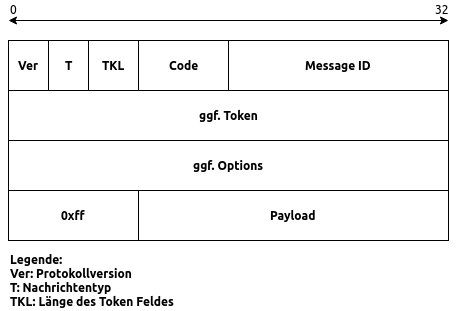
\includegraphics[width=10cm]{coappacket}
  \caption{CoAP Message Format} 
  \label{Analyse:CoAP Message Format}
\end{figure}

\clearpage

Die Nutzung des Protokolls \ac{UDP} macht es weiterhin möglich Multicast Nachrichten im Netzwerk zu verbreiten. Dies ermöglicht das Auffinden von Ressourcen im Netzwerk und ist für \ac{M2M} Kommunikation in Industrie 4.0 Umgebungen von großer Bedeutung. \ac{CoAP} Server werden mit Hilfe ihrer \ac{URI} referenziert. Werden neue Server im Netzwerk integriert, so ist es möglich, den Server mit Hilfe eines Broad- oder Multicast im Netz oder Teilnetzen bekannt zu machen. (\cite{trapickin2013})

\ac{UDP} verhindert jedoch, dass eine Verschlüsselung der Nutzdaten über \ac{TLS} bereitgestellt werden kann. \ac{TLS} benötigt eine zuverlässige Übertagung der Pakete\footnote{TODO - in }, da es auf einer sequenziellen Integritätsprüfung\footnote{TODO - was ist das} der Daten beruht. Diese Anforderungen werden vom unzuverlässigen Datargramm \ac{UDP} nicht erfüllt. Eine Sicherung der Datenübertragung muss mit Hilfe von \ac{DTLS}\footnote{TODO - was ist DTLS} hergestellt werden.

\section{Zwischenfazit}
Das Ziel einer weitreichenden Vernetzung aller Komponenten in Industrie 4.0 Umgebungen erfordert ein hohes Maß an Kommunikation zwischen den Komponenten. Neue Industrie 4.0 Netze basieren auf etablierten Technologien wie \ac{TCP}, \ac{UDP} und \ac{IP} und deren Dienste und Übernehmen deren Eigenschaften sowie Vor- und Nachteile der unteren Ebenen des \ac{TCP}/\ac{IP} Referenzmodells. Durch die Vereinheitlichung der Netzwerkkommunikation über den \ac{IP} Stack und der Vernetzung von Industriekomponenten mit Business- und Anwendungsprozessen, spielt die Bereitstellung einer sicheren Kommunikation im Netzwerk und der Schutz der Produktionssysteme vor unbefugten Zugriffen eine zentrale Rolle.

Der Fokus der Weiterentwicklung der Kommunikation im Netzwerk liegt auf der Etablierung neuer Anwendungsprotokolle zur effizienten Nachrichtenübermittlung. Darunter zählt die umfangreichen Industrielösungen \ac{OPC UA} sowie ressourcenschonende Protokolle für integrierte Lösungen wie \ac{CoAP}. \ac{OPC UA} stellt ein zukunftsorientiertes, generisches Protokoll zur Kommunikation im Netzwerk bereit. Durch die hohe Flexibilität, welche durch die weitreichenden Anforderungen der Industrie erforderlich ist, erfordert die Umsetzung einer Infrastruktur mit diesem Protokoll ein hohes Maß an administrativem Aufwand und kann bei Fehlkonfiguration eine Schwachstelle im Netzwerk darstellen. 

Um den in \autoref{Grundlagen:Grundprinzipien der sicheren Kommunikation} genannten Schutzzielen gerecht zu werden und einen ausreichenden Schutz gegen die in \autoref{Analyse:Bedrohungen} genannten Bedrohungen bereitzustellen, muss eine sichere Datenübertragung durch das Zusammenwirken mehrerer Schichten im Netzwerkstack hergestellt werden.

Im folgenden Teil der Thesis werden die in der Analyse gewonnenen Erkenntnisse und deren Auswirkungen auf das Netzwerk und dessen Kommunikation durch die Darstellung verschiedener Bedrohungsszenarien am Testsystem (\cite{Weber2018}) untersucht.